\documentclass[a4paper,10pt,openany]{article}

\usepackage[bitstream-charter]{mathdesign}
\usepackage{libertine}

\usepackage[left=19mm,right=19mm, top=2.5cm, bottom=2.9cm]{geometry}


% for proper Encoding
\usepackage[utf8]{inputenc}
\usepackage[english]{babel}

%Mathesatz
\usepackage{amsmath}
%\usepackage{amssymb}

%fancy looks:
\usepackage{microtype}

%for clickable references, much nicer to read
\usepackage{hyperref}

%for references with page numbers
\usepackage[english,vario]{fancyref}
\vrefwarning


\usepackage{graphicx}

\parindent 0pt %remove indentation for a new paragraph


%title, author
\title{Adaptive time stepping for n-body simulations}
\author{Dan Čermák}
%\date{\today}

\begin{document}

\maketitle

\section{Motivation}

\begin{figure}[h]
\begin{center}
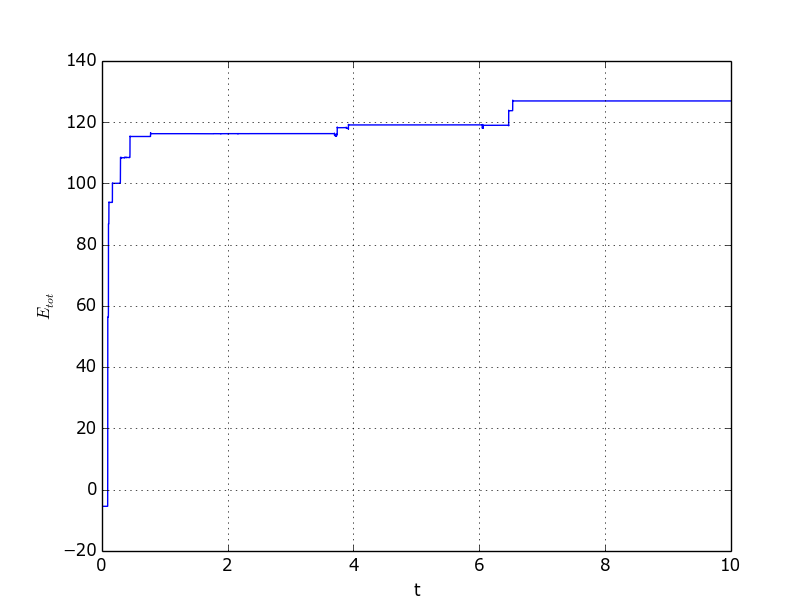
\includegraphics[width=.8\textwidth]{energy_constant_time_step.png}
\end{center}
\caption{Typical result of close encounters with too large time steps on the total energy.}\label{fig:energy constant time step}
\end{figure}

We require an adaptive time stepping routine to adjust $\Delta t$ during close encounters of two bodies. If we do not adjust it, the integrator is usually not able to correctly calculate the outcome. The typical result of too large time steps is the sudden ejection of one object or pairs of objects (depending on the mass difference). This increases the total energy of the system and thus creates wrong results. You can find an example in \fref{fig:energy constant time step}.


\section{Implementation}

There is no correct way how to implement adaptive time steps.

The most robust way is to estimate the local truncation error and adjust the time step accordingly. This however requires usually additional evaluations of the differential equation and if done incorrectly (which is by the way very easy) causes more problems then it solves.

A very common way is to estimate typical time scales of the physical system and to adjust the time step according to some empiric relation. This usually works pretty well if one is able to include all time scales in the calculation. On the downside this is usually quite tricky and requires a lot of testing.

\begin{figure}[h]
\begin{center}
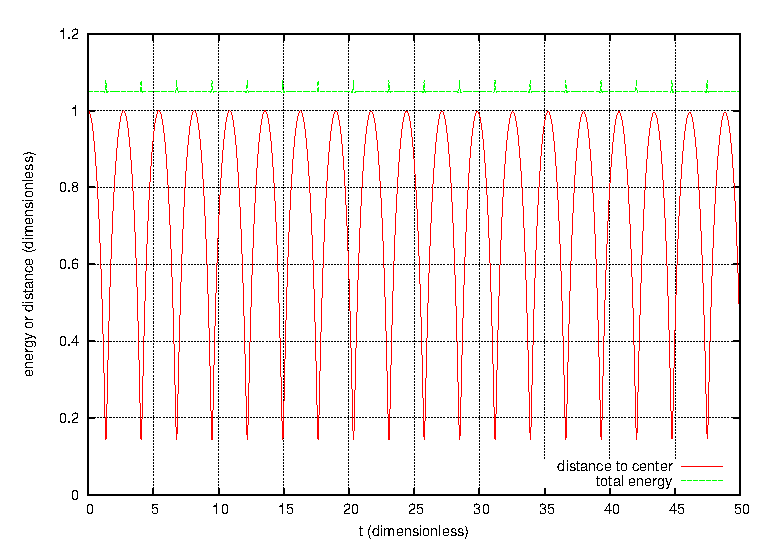
\includegraphics[width=.8\textwidth]{energy_distance.eps}
\end{center}
\caption{Simulation result with a fixed time step of the system from exercise sheet 3 task 1 a. All values are in dimensionless units as defined in task 2 a on the same exercise. The energy is multiplide by $-1200$ to fit the scale.}\label{fig:energy distance}
\end{figure}

In my opinion the easiest solution is to use the total energy of the system, as we know that it should be conserved. When using the leapfrog we might ask ourselves whether this is really an option, as the total energy is conserved. Actually the total energy is not perfectly conserved, it is just bound in a small interval as long as there are no close encounters and the time step is constant. Please consider therefore \fref{fig:energy distance}. As you can clearly see, the energy has a spike\footnote{this is actually a dip, as the energy is multiplied by a negative number} when the objects are close. We can therefore exploit the energy difference between two steps as an indicator for the distance of the objects, as we know that it will increase noticeably if the objects get close. With this we will be able to treat close encounters properly.

The actual implementation is very simple. First we have to calculate the normalized energy difference between two steps:
\begin{equation}\label{eq:energy error}
\Delta E_\mathrm{norm} = \left| \frac{E_n - E_{n-1}}{E_{n-1}} \right|
\end{equation}

If $\Delta E_\mathrm{norm}$ is larger than a threshold then:
\begin{equation}
\Delta t_\mathrm{new} = \frac{1}{2} \cdot \Delta t_\mathrm{old}
\end{equation}
Else:
\begin{equation}
\Delta t_\mathrm{new} = 2 \cdot \Delta t_\mathrm{old}
\end{equation}

Furthermore we have to ensure that $\Delta t_\mathrm{new}$ does not become too small or too large (the latter happens nearly never, the former occurs quite frequently). This is done by setting:
\begin{equation}
\Delta t_\mathrm{new} := \min(\max(\Delta t_\mathrm{new}, \text{min value}), \text{max value} )
\end{equation}

For me the following values worked:
\begin{equation}
\begin{aligned}
\text{min value} &= 10^{-10}\\
\text{max value} &= 1\\
\text{threshold} &= 10^{-10}
\end{aligned}
\end{equation}

You can see an example in \fref{fig:adaptive time stepping}. As you can clearly see, the adaptive time stepping treats the close encounters properly and the total energy stays bound.

\begin{figure}
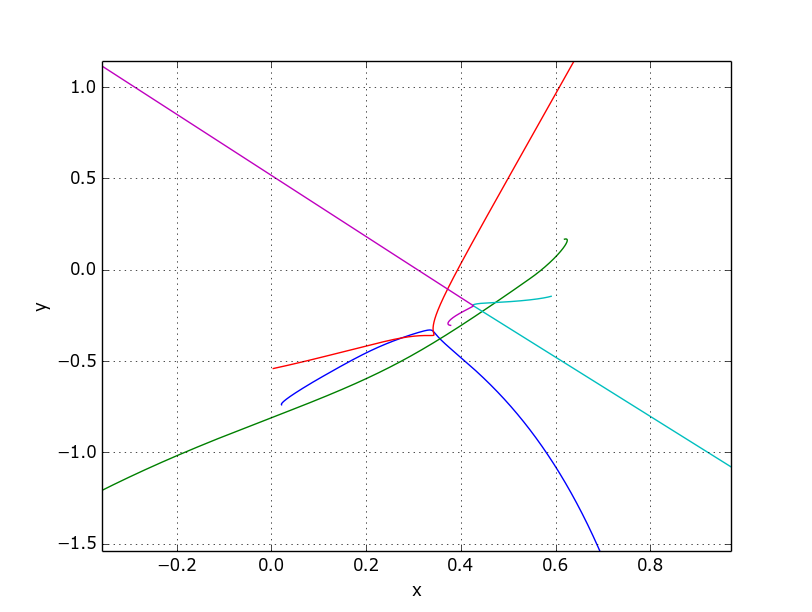
\includegraphics[width=.5\textwidth]{5_bodies_constant_step.png}
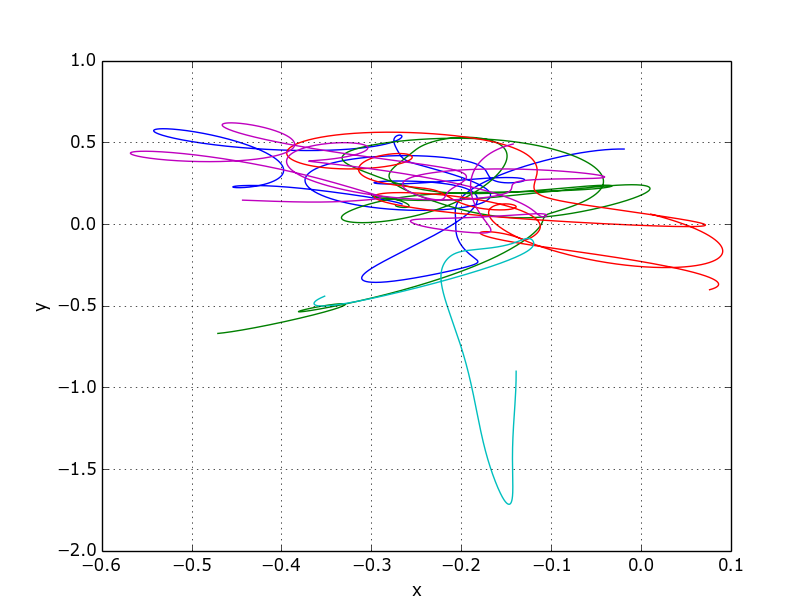
\includegraphics[width=.5\textwidth]{5_bodies_adaptive_step.png}\\
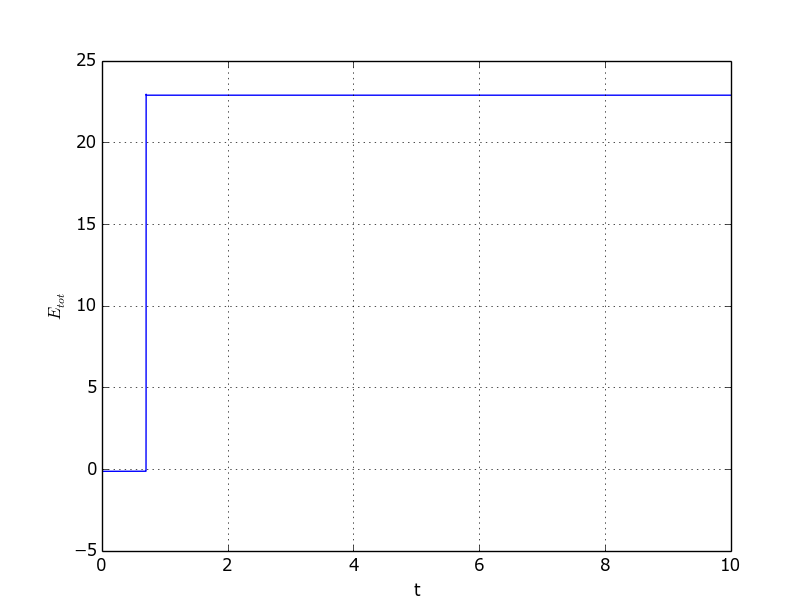
\includegraphics[width=.5\textwidth]{5_bodies_constant_step_energy.png}
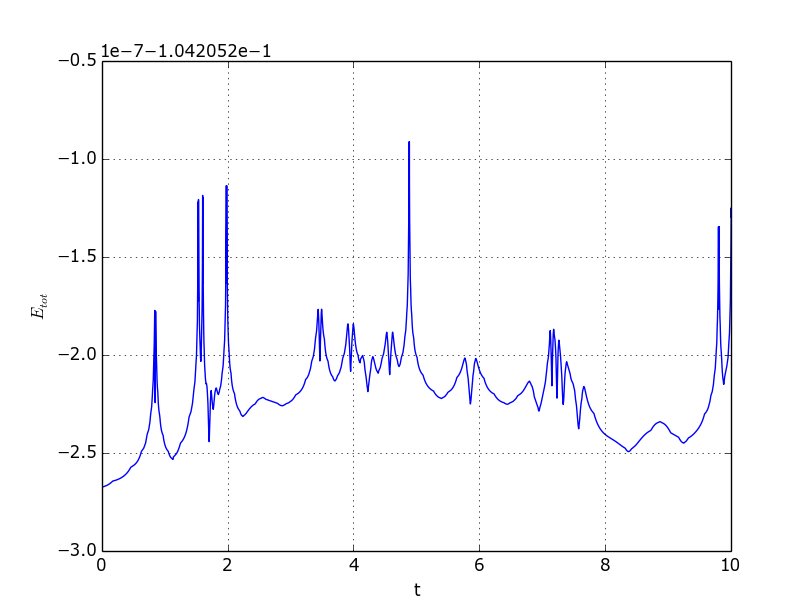
\includegraphics[width=.5\textwidth]{5_bodies_adaptive_step_energy.png}
\caption{Simulation of 5 objects at random initial positions (like in exercise 2 e, sheet 3) simulated with adaptive and constant time stepping. The upper left image shows the positions in the x-y plane of the objects with a constant time step, whereas the image beside it shows the same but with adaptive time steps (the initial conditions are different, but only the qualitative result is interesting). The lower row shows the energy as a function of time for the same runs as in the images above.}\label{fig:adaptive time stepping}
\end{figure}


\section{Additional considerations}

\subsection{Energy error}

The calculation of the energy error in \fref{eq:energy error} has the problem, that it will create a \verb|NaN| if $E_{n-1}$ is exactly zero. As that is unlikely, no special treatment has been done.

One could however check whether $E_{n-1}$ is zero and in that case choose a reasonable value for the normalized difference (for instance $1$ if one replaces the denominator of \fref{eq:energy error} by $E_n$).

\subsection{Additional threshold}

It might not be very smart to refine the time step every time (as it is done currently). One could for instance introduce an interval in which the time step remains unchanged and only refine it if it falls out of this interval. For simplicity this was not implemented and thus not tested, therefore no guarantee that it works.

\subsection{Long term evolution}

When one changes the time step, the symplectic behavior of the leapfrog is partially lost. Thus an overall energy drift can happen. This is the price one has to pay for treating close encounters (now you can also imagine why big n-body simulations have high precision solvers for the close encounters but use low order solvers for the remaining time). You can see this in \fref{fig:adaptive time stepping long time}.

\begin{figure}
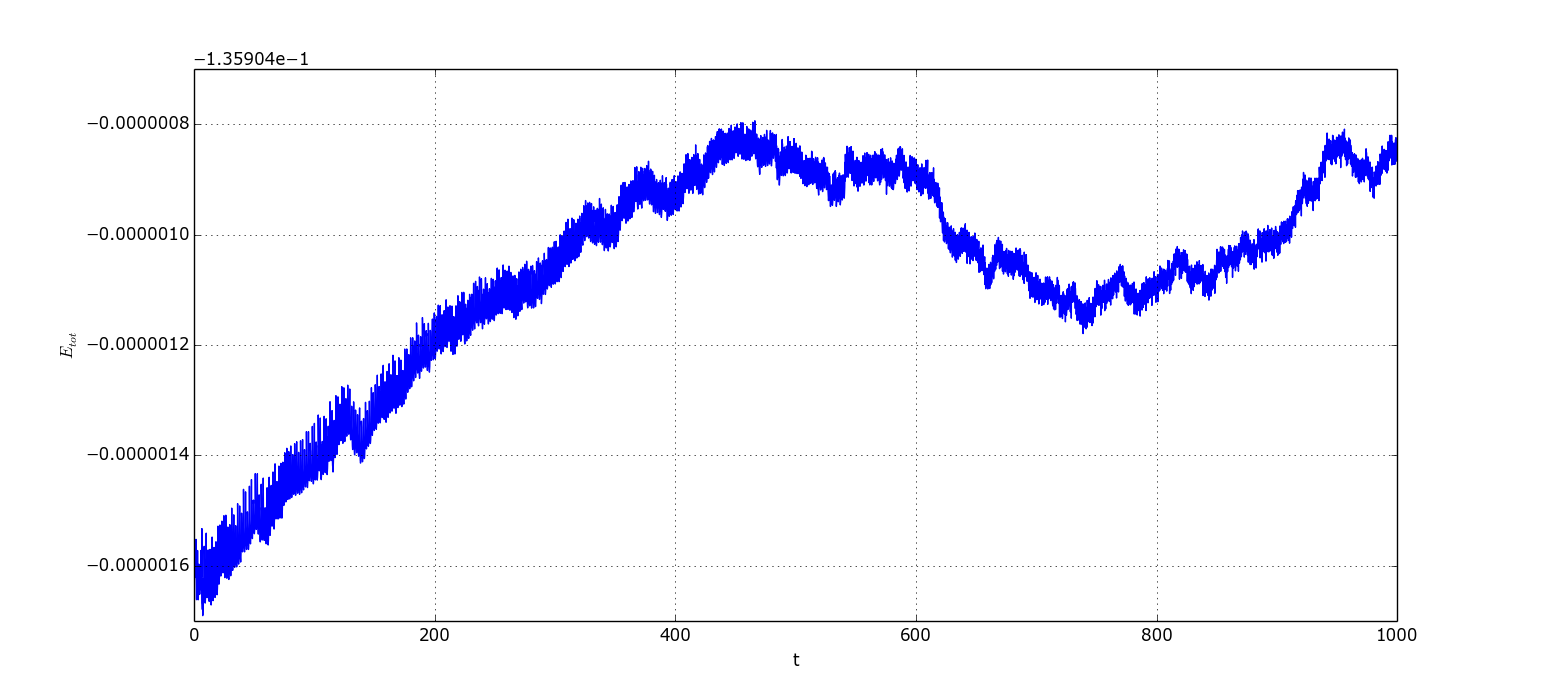
\includegraphics[width=\textwidth]{5_bodies_adaptive_step_energy_long_time.png}
\caption{Simulation of 5 objects at random initial positions (like in exercise 2 e, sheet 3) simulated with adaptive time stepping. The plot shows the total energy as a function of time. As you can see there is an overall energy drift even though the leapfrog algorithm was used.}\label{fig:adaptive time stepping long time}
\end{figure}
 
\end{document}